


\tikzset{every picture/.style={line width=0.75pt}} %set default line width to 0.75pt

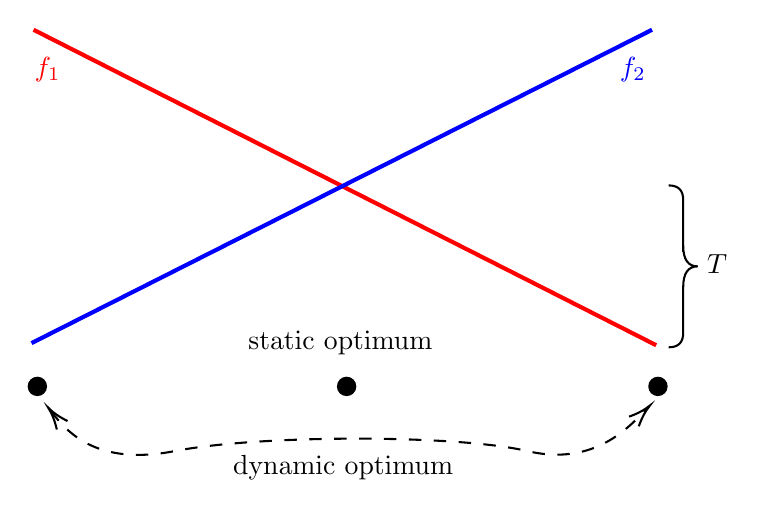
\begin{tikzpicture}[x=0.75pt,y=0.75pt,yscale=-1,xscale=1]
%uncomment if require: \path (0,300); %set diagram left start at 0, and has height of 300

%Shape: Circle [id:dp3024076819219861]
\draw  [fill=black  ,fill opacity=1 ] (305.67,223.17) .. controls (305.67,220.87) and (307.53,219) .. (309.83,219) .. controls (312.13,219) and (314,220.87) .. (314,223.17) .. controls (314,225.47) and (312.13,227.33) .. (309.83,227.33) .. controls (307.53,227.33) and (305.67,225.47) .. (305.67,223.17) -- cycle ;
%Shape: Circle [id:dp7041225921361765]
\draw  [fill=black  ,fill opacity=1 ] (156.67,223.17) .. controls (156.67,220.87) and (158.53,219) .. (160.83,219) .. controls (163.13,219) and (165,220.87) .. (165,223.17) .. controls (165,225.47) and (163.13,227.33) .. (160.83,227.33) .. controls (158.53,227.33) and (156.67,225.47) .. (156.67,223.17) -- cycle ;
%Shape: Circle [id:dp8996341089567816]
\draw  [fill=black  ,fill opacity=1 ] (455.67,223.17) .. controls (455.67,220.87) and (457.53,219) .. (459.83,219) .. controls (462.13,219) and (464,220.87) .. (464,223.17) .. controls (464,225.47) and (462.13,227.33) .. (459.83,227.33) .. controls (457.53,227.33) and (455.67,225.47) .. (455.67,223.17) -- cycle ;
%Curve Lines [id:da9487169876590669]
\draw [line width=0.75]  [dash pattern={on 4.5pt off 4.5pt}]  (167.3,235) .. controls (174.51,244.28) and (188.46,261.85) .. (227,254.33) .. controls (268,246.33) and (363,246.33) .. (397,254.33) .. controls (429.3,261.93) and (446.27,242.44) .. (454.73,233.63) ;
\draw [shift={(456,232.33)}, rotate = 495] [color=black  ][line width=0.75]    (10.93,-3.29) .. controls (6.95,-1.4) and (3.31,-0.3) .. (0,0) .. controls (3.31,0.3) and (6.95,1.4) .. (10.93,3.29)   ;
\draw [shift={(166,233.33)}, rotate = 51.55] [color=black  ][line width=0.75]    (10.93,-3.29) .. controls (6.95,-1.4) and (3.31,-0.3) .. (0,0) .. controls (3.31,0.3) and (6.95,1.4) .. (10.93,3.29)   ;
%Straight Lines [id:da002446124086751267]
\draw [color=red  ,draw opacity=1 ][line width=1.5]    (159,51.33) -- (459,203.33) ;
%Straight Lines [id:da715905705967314]
\draw [color=blue  ,draw opacity=1 ][line width=1.5]    (158,202.33) -- (457,51.33) ;
%Shape: Brace [id:dp3550286018056783]
\draw  [line width=0.75]  (465,204.33) .. controls (469.67,204.33) and (472,202) .. (472,197.33) -- (472,175.33) .. controls (472,168.66) and (474.33,165.33) .. (479,165.33) .. controls (474.33,165.33) and (472,162) .. (472,155.33)(472,158.33) -- (472,133.33) .. controls (472,128.66) and (469.67,126.33) .. (465,126.33) ;

% Text Node
\draw (240,255) node [anchor=north west][inner sep=0.75pt]   [align=left] {\begin{minipage}[lt]{100pt}\setlength\topsep{0pt}
\begin{center}
dynamic optimum
\end{center}

\end{minipage}};
% Text Node
\draw (252,195) node [anchor=north west][inner sep=0.75pt]   [align=left] {\begin{minipage}[lt]{80pt}\setlength\topsep{0pt}
\begin{center}
static optimum
\end{center}

\end{minipage}};
% Text Node
\draw (158,63) node [anchor=north west][inner sep=0.75pt]  [color=red  ,opacity=1 ]  {$f_{1}$};
% Text Node
\draw (440,63) node [anchor=north west][inner sep=0.75pt]  [color=blue  ,opacity=1 ]  {$f_{2}$};
% Text Node
\draw (482,158) node [anchor=north west][inner sep=0.75pt]    {$T$};


\end{tikzpicture}
